% Copyright 2004 by Till Tantau <tantau@users.sourceforge.net>.
%
% In principle, this file can be redistributed and/or modified under
% the terms of the GNU Public License, version 2.
%
% However, this file is supposed to be a template to be modified
% for your own needs. For this reason, if you use this file as a
% template and not specifically distribute it as part of a another
% package/program, I grant the extra permission to freely copy and
% modify this file as you see fit and even to delete this copyright
% notice. 

\documentclass[aspectratio=169]{beamer}
%\documentclass{beamer}

\setbeamersize{text margin left=5mm, text margin right=5mm}


\defbeamertemplate{headline}{my header}{%
\vskip1pt%
\makebox[0pt][l]{\,\insertshortauthor}%
\hspace*{\fill}\insertshorttitle/\insertshortsubtitle\hspace*{\fill}%
\llap{\insertpagenumber/\insertpresentationendpage\,}
}
\setbeamertemplate{headline}[my header]

\let\olditem\item
\renewcommand{\item}{\setlength{\itemsep}{\fill}\olditem}

\usepackage{soul}
\usepackage{tkz-euclide}
\usetikzlibrary{calc}
\usepackage[]{algorithm2e}
\usepackage{changepage}
\usepackage{amssymb}
\usepackage{xcolor}
\usepackage{mathtools}
\usepackage{tcolorbox}
\usepackage{tikz}
\usepackage{tikz-3dplot}
\usepackage[export]{adjustbox}
\usepackage{tabu}

% \usepackage[math]{cellspace}
% \cellspacetoplimit 4pt
% \cellspacebottomlimit 4pt
%\usetikzlibrary{arrows.meta}

%\setbeamertemplate{itemize items}{-}

%\usepackage{helvet}
\usefonttheme{professionalfonts} % using non standard fonts for beamer
%\usefonttheme{serif} % default family is serif
%\usepackage{fontspec}
%\setmainfont{Liberation Serif}

% There are many different themes available for Beamer. A comprehensive
% list with examples is given here:
% http://deic.uab.es/~iblanes/beamer_gallery/index_by_theme.html
% You can uncomment the themes below if you would like to use a different
% one:
%\usetheme{AnnArbor}
%\usetheme{Antibes}
%\usetheme{Bergen}
%\usetheme{Berkeley}
%\usetheme{Berlin}
%\usetheme{Boadilla}
%\usetheme{boxes}
%\usetheme{CambridgeUS}
%\usetheme{Copenhagen}
%\usetheme{Darmstadt}
%\usetheme{default}
%\usetheme{Frankfurt}
%\usetheme{Goettingen}
%\usetheme{Hannover}
%\usetheme{Ilmenau}
%\usetheme{JuanLesPins}
%\usetheme{Luebeck}
%\usetheme{Madrid}
%\usetheme{Malmoe}
%\usetheme{Marburg}
%\usetheme{Montpellier}
%\usetheme{PaloAlto}
%\usetheme{Pittsburgh}
%\usetheme{Rochester}
%\usetheme{Singapore}
%\usetheme{Szeged}
%\usetheme{Warsaw}


\def\mf{\ensuremath\mathbf}
\def\mb{\ensuremath\mathbb}
\def\lp{\ensuremath\left(}
\def\rp{\ensuremath\right)}
\def\lv{\ensuremath\left\lvert}
\def\rv{\ensuremath\right\rvert}
\def\lV{\ensuremath\left\lVert}
\def\rV{\ensuremath\right\rVert}
\def\lc{\ensuremath\left\{}
\def\rc{\ensuremath\right\}}
\def\ls{\ensuremath\left[}
\def\rs{\ensuremath\right]}
\def\bmx{\ensuremath\begin{bmatrix*}[r]}
\def\emx{\ensuremath\end{bmatrix*}}
\def\bmxc{\ensuremath\begin{bmatrix*}[c]}
\def\t{\lp t\rp}
\def\k{\ls k\rs}


\newcommand{\demoex}[2]{\onslide<#1->\begin{color}{black!60} #2 \end{color}}
\newcommand{\demoexc}[3]{\onslide<#1->\begin{color}{#2} #3 \end{color}}
\newcommand{\anim}[3]{\onslide<#1->{\begin{color}{#2!60} #3 \end{color}}}
\newcommand{\ct}[1]{\lp #1\rp}
\newcommand{\dt}[1]{\ls #1\rs}
\newcommand{\cols}[2]{\begin{columns}[#1] #2 \end{columns}}
\newcommand{\col}[2]{\begin{column}{#1} #2 \end{column}}


\title{Introduction to Digital Signal Processing}

% A subtitle is optional and this may be deleted
\subtitle{Linear Time-Invariant Systems}

\author{Sivakumar Balasubramanian}
% - Give the names in the same order as the appear in the paper.
% - Use the \inst{?} command only if the authors have different
%   affiliation.

\institute[Christian Medical College] % (optional, but mostly needed)
{
  \inst{}%
  Department of Bioengineering\\
  Christian Medical College, Bagayam\\
  Vellore 632002
}
% - Use the \inst command only if there are several affiliations.
% - Keep it simple, no one is interested in your street address.

\date{}
% - Either use conference name or its abbreviation.
% - Not really informative to the audience, more for people (including
%   yourself) who are reading the slides online

\subject{Lecture slides on Introduction to DSP}
% This is only inserted into the PDF information catalog. Can be left
% out. 

% If you have a file called "university-logo-filename.xxx", where xxx
% is a graphic format that can be processed by latex or pdflatex,
% resp., then you can add a logo as follows:

% \pgfdeclareimage[height=0.5cm]{university-logo}{university-logo-filename}
% \logo{\pgfuseimage{university-logo}}

% Delete this, if you do not want the table of contents to pop up at
% the beginning of each subsection:
\AtBeginSubsection[]
{
  \begin{frame}<beamer>{Outline}
    \tableofcontents[currentsection,currentsubsection]
  \end{frame}
}

% Let's get started
\begin{document}

\begin{frame}
  \titlepage
\end{frame}

\begin{frame}[t]{Input-Output Relationship of System}
\begin{figure}
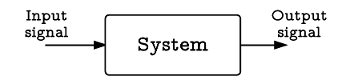
\includegraphics[width=0.6\textwidth]{img/system.png}
\end{figure}
\end{frame}

\begin{frame}[t]{Input-Output Relationship of Linear System}
\textbf{Linearity}:
\[ x_i[n] \mapsto y_i[n] \implies \sum_{i} \alpha_i x_i[n] \mapsto \sum_{i} \alpha_i y_i[n] \]
\end{frame}

\begin{frame}[t]{Input-Output Relationship of Time-Invariant System}
\textbf{Time-invariance}:  
\[ x_i[n] \mapsto y_i[n] \implies x_i[n - k] \mapsto y_i[n-k] \]
\end{frame}

\begin{frame}[t]{Linear Time Invariant (LTI) System}
\textbf{Input-Output Relationship}
\[ x_i[n] \mapsto y_i[n] \implies \sum_{i} \alpha_i x_i[n - k_i] \mapsto \sum_{i} \alpha_i y_i[n - k_i] \]
\end{frame}

\begin{frame}[t]{Importance of the Impulse Signal}
Any signal $x[n]$ can be represented as a linear combinration of time-shifted impulse signals.
\[ x[n]  = \sum_{k=-\infty}^{\infty} x[k] \delta[n - k] \]
\begin{figure}
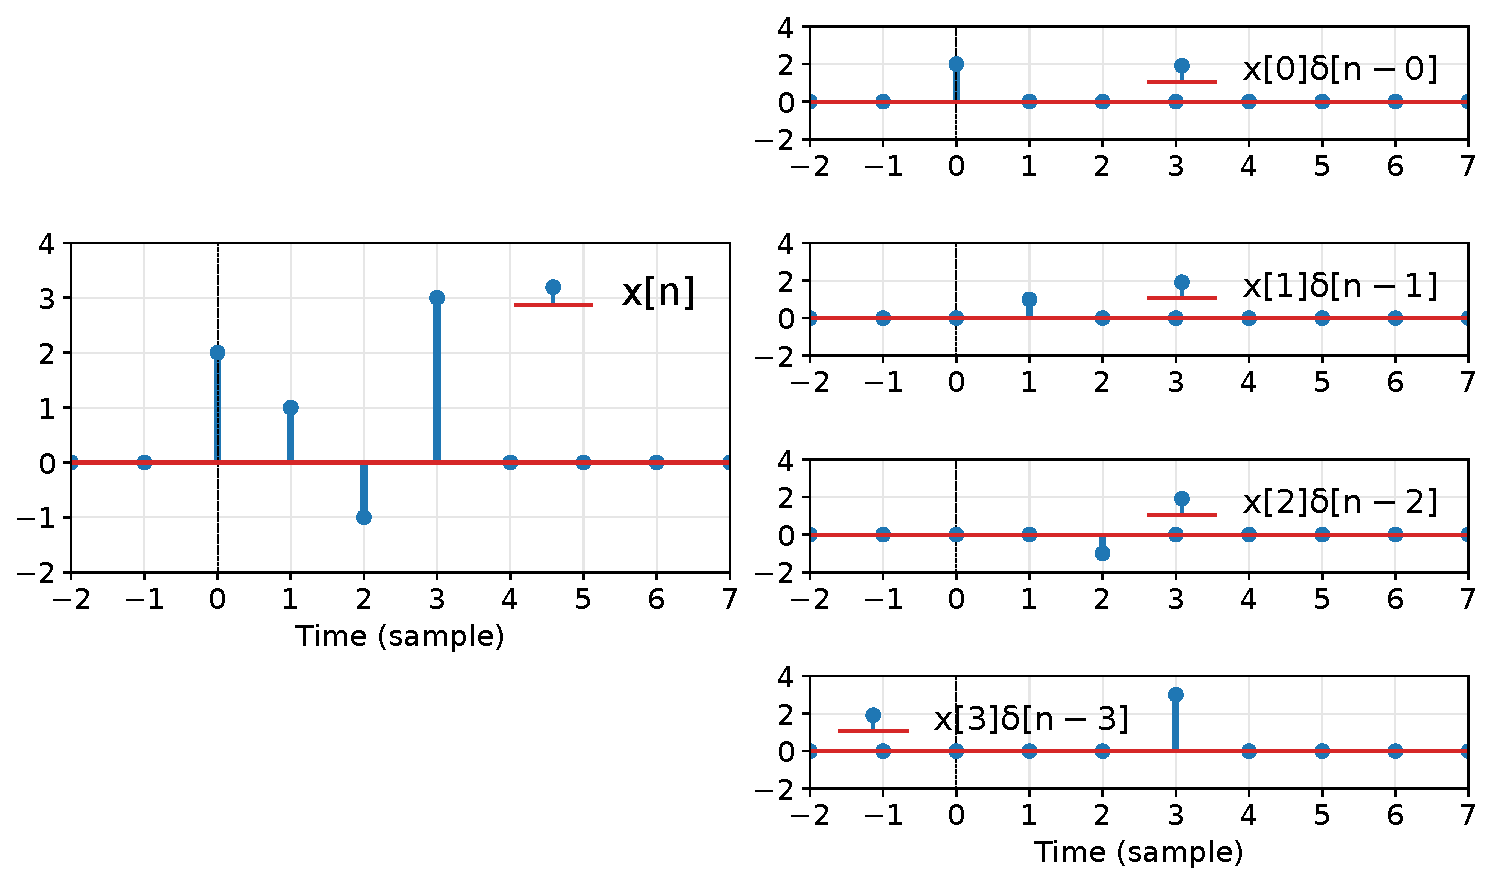
\includegraphics[width=0.6\textwidth]{img/sigimpdecomp.eps}
\end{figure}
\end{frame}

\begin{frame}[t]{Impulse Response of an LTI System}
\textbf{Impulse Response}: The response of an LTI system to an impulse input.

\[ h[n]  = \mathcal{H}\left( \delta[n] \right) \]

If we know this, then we know the following for an LTI system:
\[ \delta[n] \mapsto h[n] \implies \begin{cases}
\delta[n - k] &\mapsto h[n - k] \\
\alpha_k \cdot \delta[n - k] &\mapsto \alpha_k \cdot h[n - k] \\
\sum_k \alpha_k \cdot \delta[n - k] &\mapsto \sum_k\alpha_k \cdot h[n - k]
\end{cases} \]

\[ x[n] =\sum_k x[k] \cdot \delta[n - k] \xrightarrow{\quad \mathcal{H} \quad} \sum_k x[k] \cdot h[n - k] = x[n] * h[n] \]
\end{frame}

\begin{frame}[t]{Output of an LTI System}
\begin{figure}
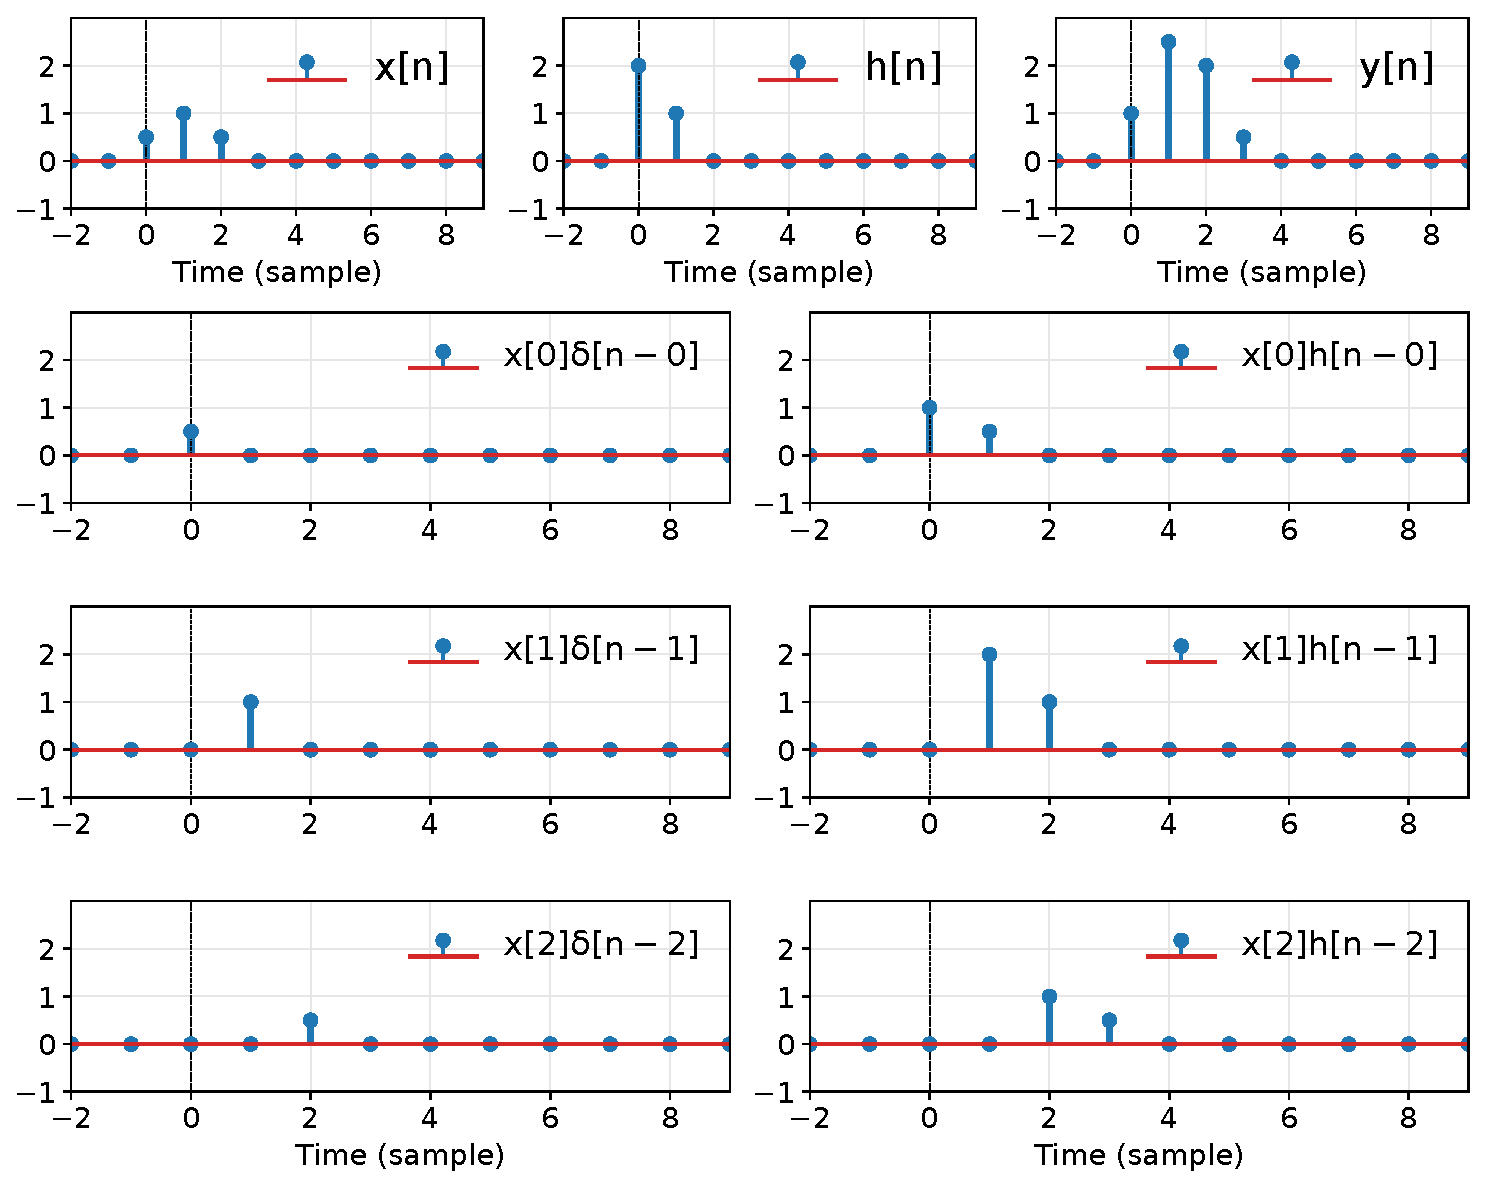
\includegraphics[width=0.6\textwidth]{img/convdemo1.eps}
\end{figure}
\end{frame}

\begin{frame}[t]{Convolution Sum}
\begin{Large}
\[ y[n] = x[n] * h[n] = \sum_k x[k] \cdot h[n - k] \]
\end{Large}
\end{frame}

\begin{frame}[t]{Alternative View of the Convolution Sum}
\begin{Large}
\[ y[n] = x[n] * h[n] = \sum_k x[k] \cdot h[n - k] \]
\end{Large}
\begin{center}
\begin{tabu}{c|c|c|c|c|c|c|c|c|c|c|c|c|c}
\hline
$k$ & $\cdots$ & -3 &  -2 & -1 & 0 & 1 & 2 & 3 & 4 & 5 & 6 & 7 & $\cdots$ \\ \hline
\rowfont{\color{red}} $x[k]$ & $\cdots$ & 0 & 0 & 0 & 0.5 & 1 & 0.5 & 0 & 0 & 0 & 0 & $\cdots$ &  \\ \hline
$h[\quad - k]$ & $\cdots$ &  &  &  &  &  &  &  &  &  &  &  & $\cdots$ \\ \hline
$h[\quad - k]$ & $\cdots$ &  &  &  &  &  &  &  &  &  &  &  & $\cdots$ \\ \hline
$h[\quad - k]$ & $\cdots$ &  &  &  &  &  &  &  &  &  &  &  & $\cdots$ \\ \hline
$h[\quad - k]$ & $\cdots$ &  &  &  &  &  &  &  &  &  &  &  & $\cdots$ \\ \hline
$h[\quad - k]$ & $\cdots$ &  &  &  &  &  &  &  &  &  &  &  & $\cdots$ \\ \hline
$h[\quad - k]$ & $\cdots$ &  &  &  &  &  &  &  &  &  &  &  & $\cdots$ \\ \hline
$h[\quad - k]$ & $\cdots$ &  &  &  &  &  &  &  &  &  &  &  & $\cdots$ \\ \hline
\end{tabu}
\end{center}
\end{frame}

\begin{frame}[t]{What does the impulse response tell us?}
\[
\begin{split}
y[n] &= x[n] * h[n] = \sum_k x[k] \cdot h[n - k] \\
     &= h[n] * x[n] = \sum_k h[k] \cdot x[n - k] \\
     &= \cdots + h[2] \cdot x[n-2] + h[1] \cdot x[n-1] \\
     &\quad \quad \,\,\, + h[0] \cdot x[n]\\
     &\quad \quad \,\,\, + h[-1] \cdot x[n + 1] + h[-2] \cdot x[n + 2] + \cdots
\end{split}
\]

\end{frame}

% \begin{frame}{What is a system?}
% \begin{figure}
% 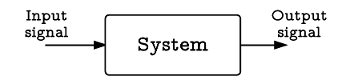
\includegraphics[width=0.6\textwidth]{img/system.png}
% \end{figure}
% Can be thought of a mapping function. \textit{e.g.}
% \[ y[n] = \mathcal{H}\left(x[n]\right) \]
% \end{frame}

% % OPERATIONS ON SIGNALS
% \begin{frame}[t]{Operations on signals}

% \begin{columns}[t]
%   \begin{column}{.45\linewidth}
%   \textbf{Operations on the dependent variable}
%   \begin{itemize}
%     \item \textbf{Scaling}: $y\ls n \rs = a \cdot x\ls n \rs$
%     \item \textbf{Addition}: $y\ls n \rs = x_1\ls n \rs + x_2\ls n \rs$
%   \end{itemize}
%   \end{column}

%   \begin{column}{.48\linewidth}
%   \textbf{Operations on the independent variable}
%   \begin{itemize}
%     \item \textbf{Time shifting}: $y\ls n \rs = x \ls n - k \rs, k \in \mathbb{Z}$
%     \item \textbf{Time reversal}: $y\ls n \rs = x \ls -n \rs, k \in \mathbb{Z}$
%   \end{itemize}
%   \end{column}
% \end{columns}

% \end{frame}

% % TIME SHIFTING
% \begin{frame}{Operation on the independent variable: \textbf{Time shifting}}

% Consider $x\ls n \rs$ shown below,

% \begin{figure}
% 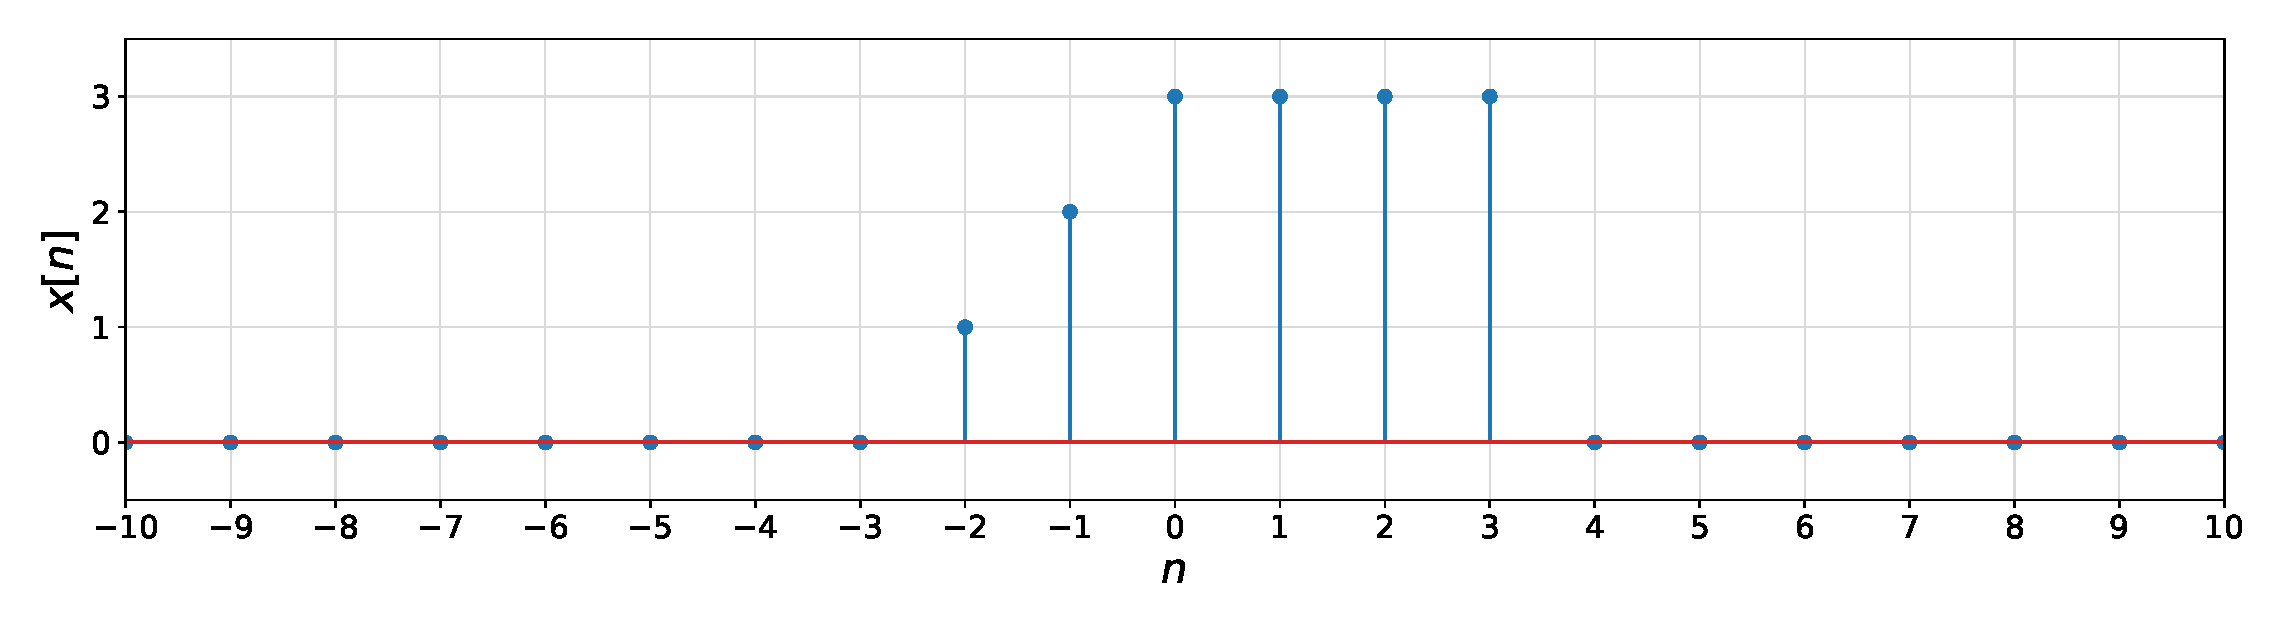
\includegraphics[width=\textwidth]{img/discsig.eps}
% \end{figure}

% What does $x\ls n - 3\rs$ look like?
% \end{frame}

% % TIME SHIFTING
% \begin{frame}{Operation on the independent variable: \textbf{Time shifting}}

% $x\ls n - 3\rs$ 

% \begin{figure}
% 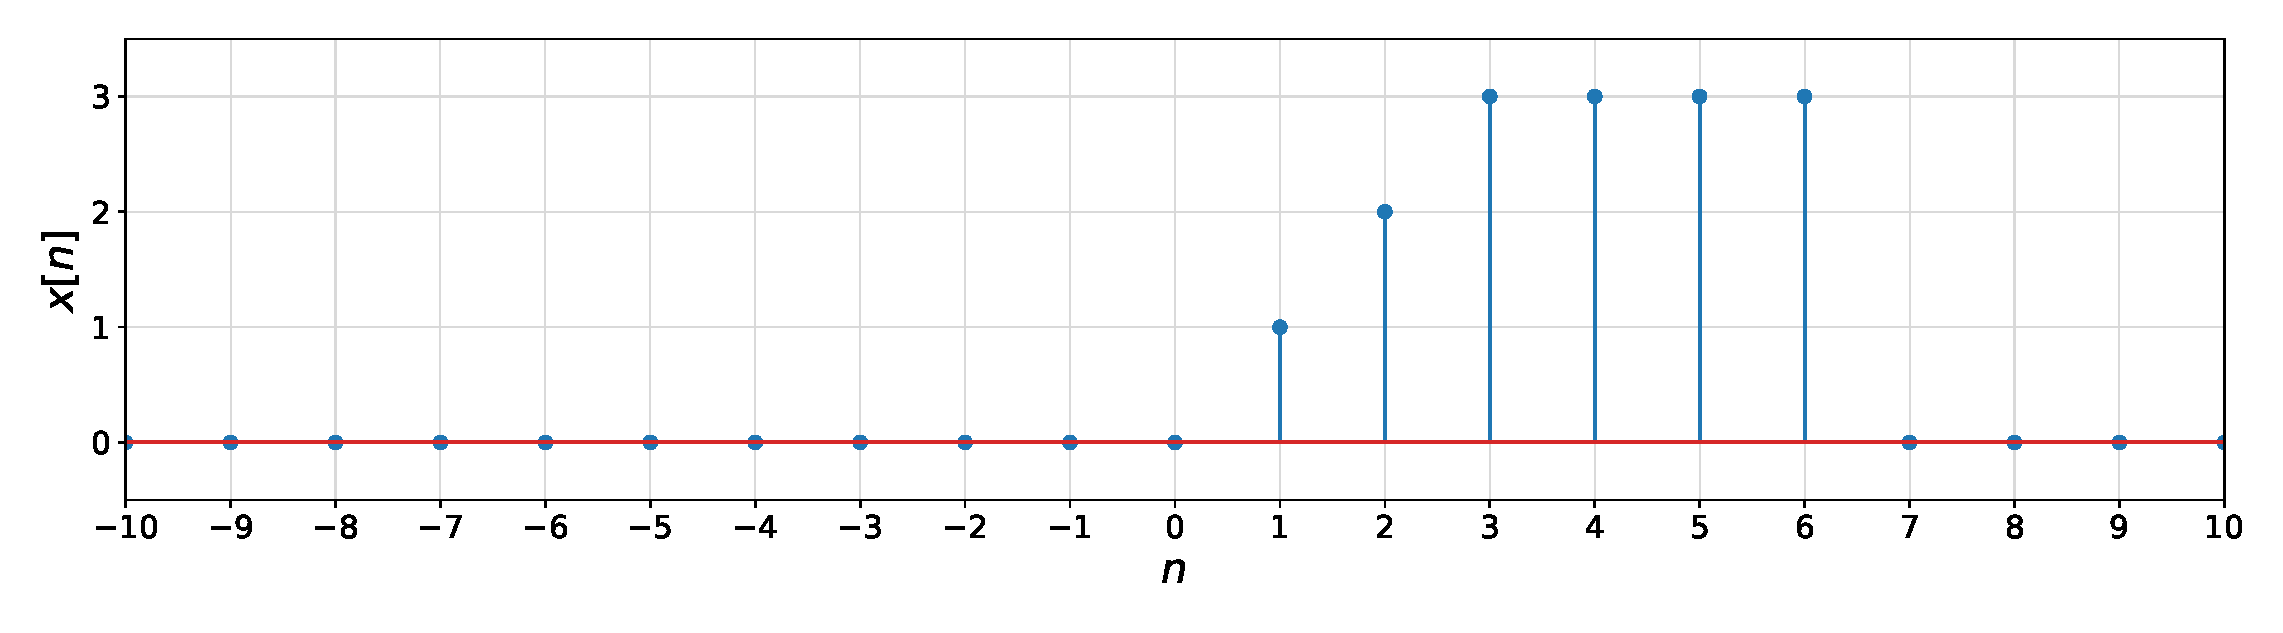
\includegraphics[width=\textwidth]{img/discsig-shift.eps}
% \end{figure}

% What about $x\ls n + 2\rs$?

% \end{frame}

% % TIME SHIFTING
% \begin{frame}{Operation on the independent variable: \textbf{Time shifting}}

% $x\ls n + 2 \rs$ 

% \begin{figure}
% 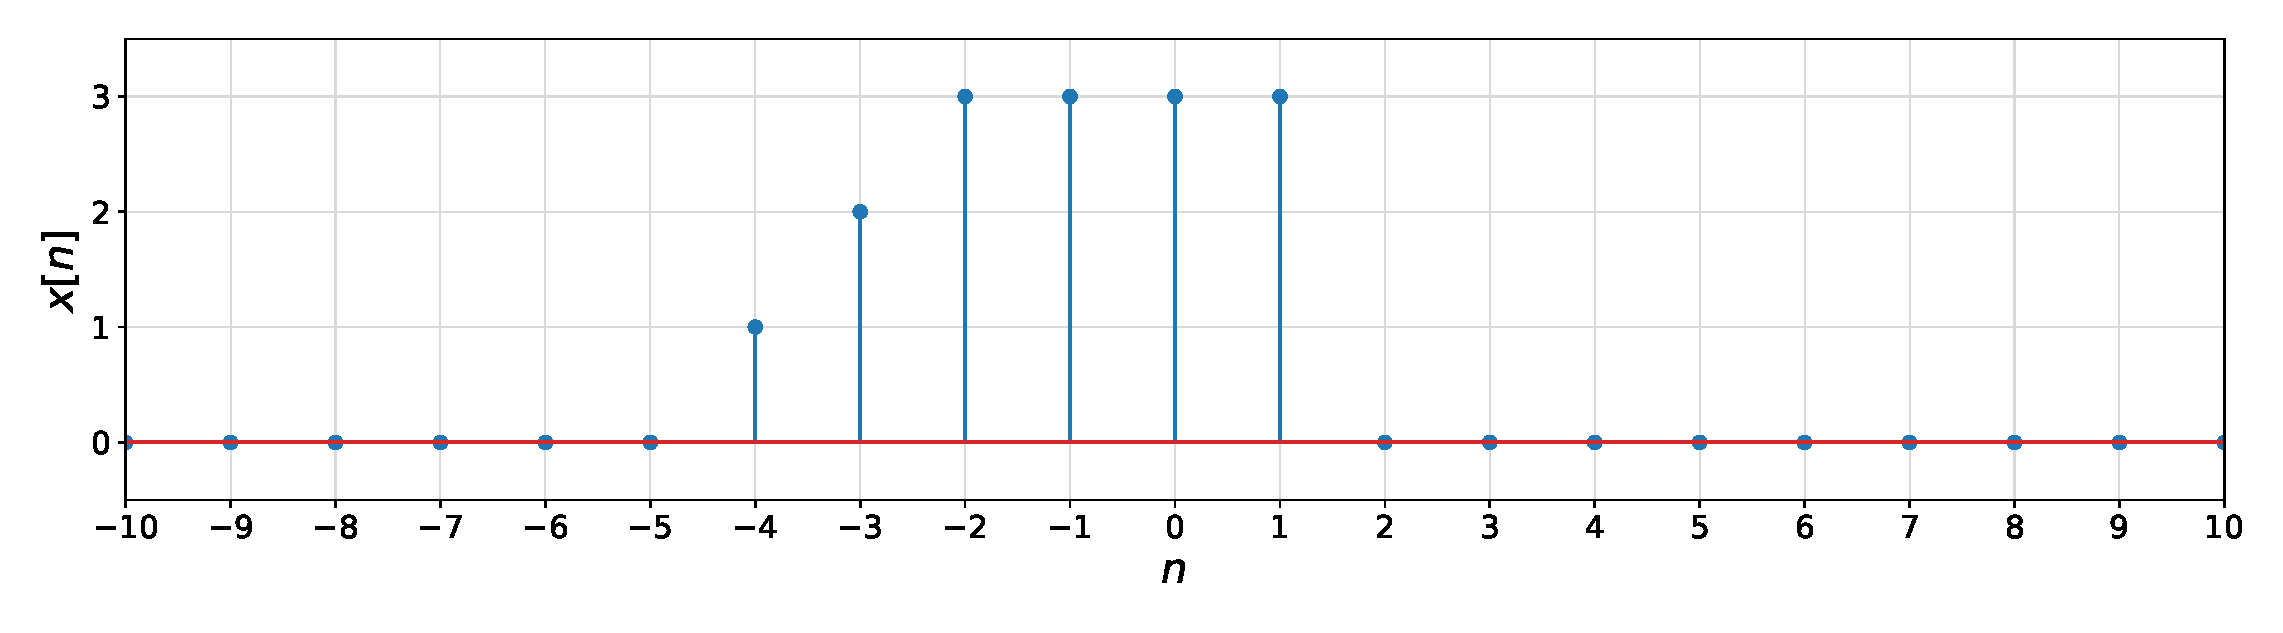
\includegraphics[width=\textwidth]{img/discsig-shift2.eps}
% \end{figure}

% \end{frame}

% % TIME Reversal
% \begin{frame}{Operation on the independent variable: \textbf{Time reversal}}

% $x\ls -n \rs$ 

% \begin{figure}
% 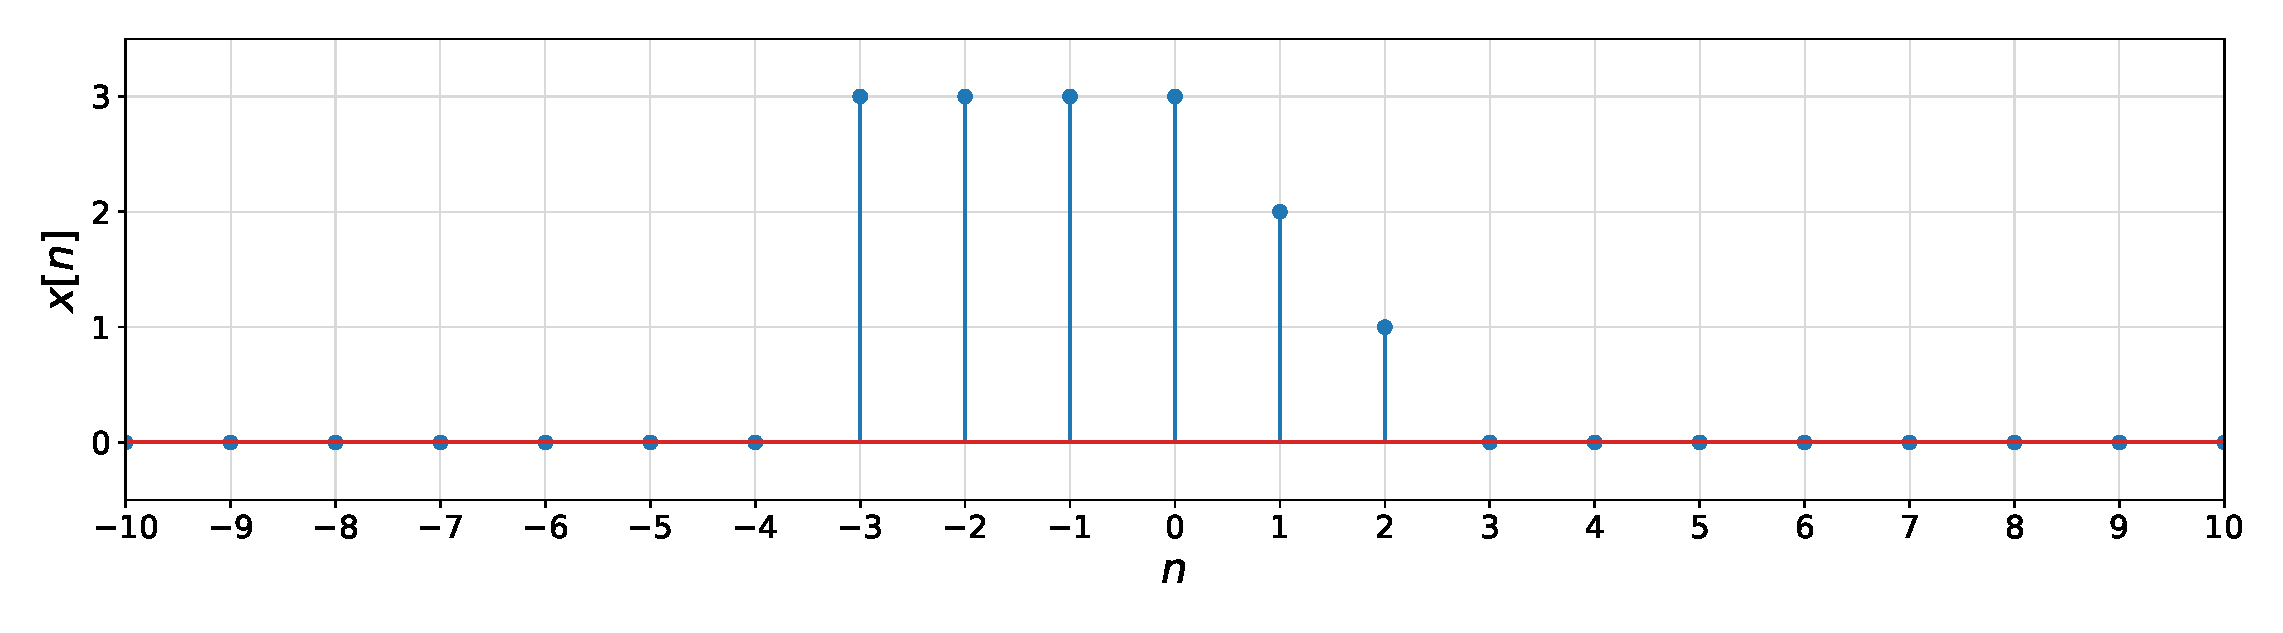
\includegraphics[width=\textwidth]{img/discsig-inv.eps}
% \end{figure}

% And $x\ls -n\rs$?

% \end{frame}


% \begin{frame}{Classification of systems}

% Based on the properties of the system.

% \begin{itemize}
% \item \textbf{Linearity}: \textit{satisfies the properties of \textbf{scaling} and \textbf{superposition}}.

% Let us assume, 
% \[ \mathcal{H}: x_i\ls n \rs \mapsto y_i\ls n \rs \]

% The system $\mathcal{H}$ is linear, if and only if,
% \[ \mathcal{H}:\sum_ia_ix_i\ls n \rs \mapsto \sum_ia_iy_i\ls n \rs \]

% \textit{Which of these systems are linear?}
% \begin{enumerate}
% \item $y\ls n \rs = k_1x\ls n \rs + k_2x\ls t-2 \rs$
% \item $y\ls n \rs = \sum_{k=n-N}^{n}x \ls k \rs $
% \item $y\ls n \rs = 0.5x\ls n \rs + 1.5$
% \end{enumerate}
% \end{itemize}
% \end{frame}

% % CLASSIFICATION OF SYSTEMS
% \begin{frame}[t]{Classification of systems}

% % Based on the properties of the system.

% \begin{itemize}
% \item \textbf{Memory}: \textit{a system whose output depends on past or future values of its input is a system with memory, else the system is memoryless}. 

% Note: the system may or may not depends on its present.

% \[ \begin{cases}
% y\ls n \rs = 0.5x\ls n \rs & \mathrm{\textbf{Memoryless system}} \\
% y\ls n \rs = \sum_{k=m_1}^{m_2} x\ls n - k\rs & \mathrm{\textbf{System with memory}}
% \end{cases}
% \]
% \end{itemize}

% \end{frame}

% % CLASSIFICATION OF SYSTEMS
% \begin{frame}[t]{Classification of systems}

% \begin{figure}
% 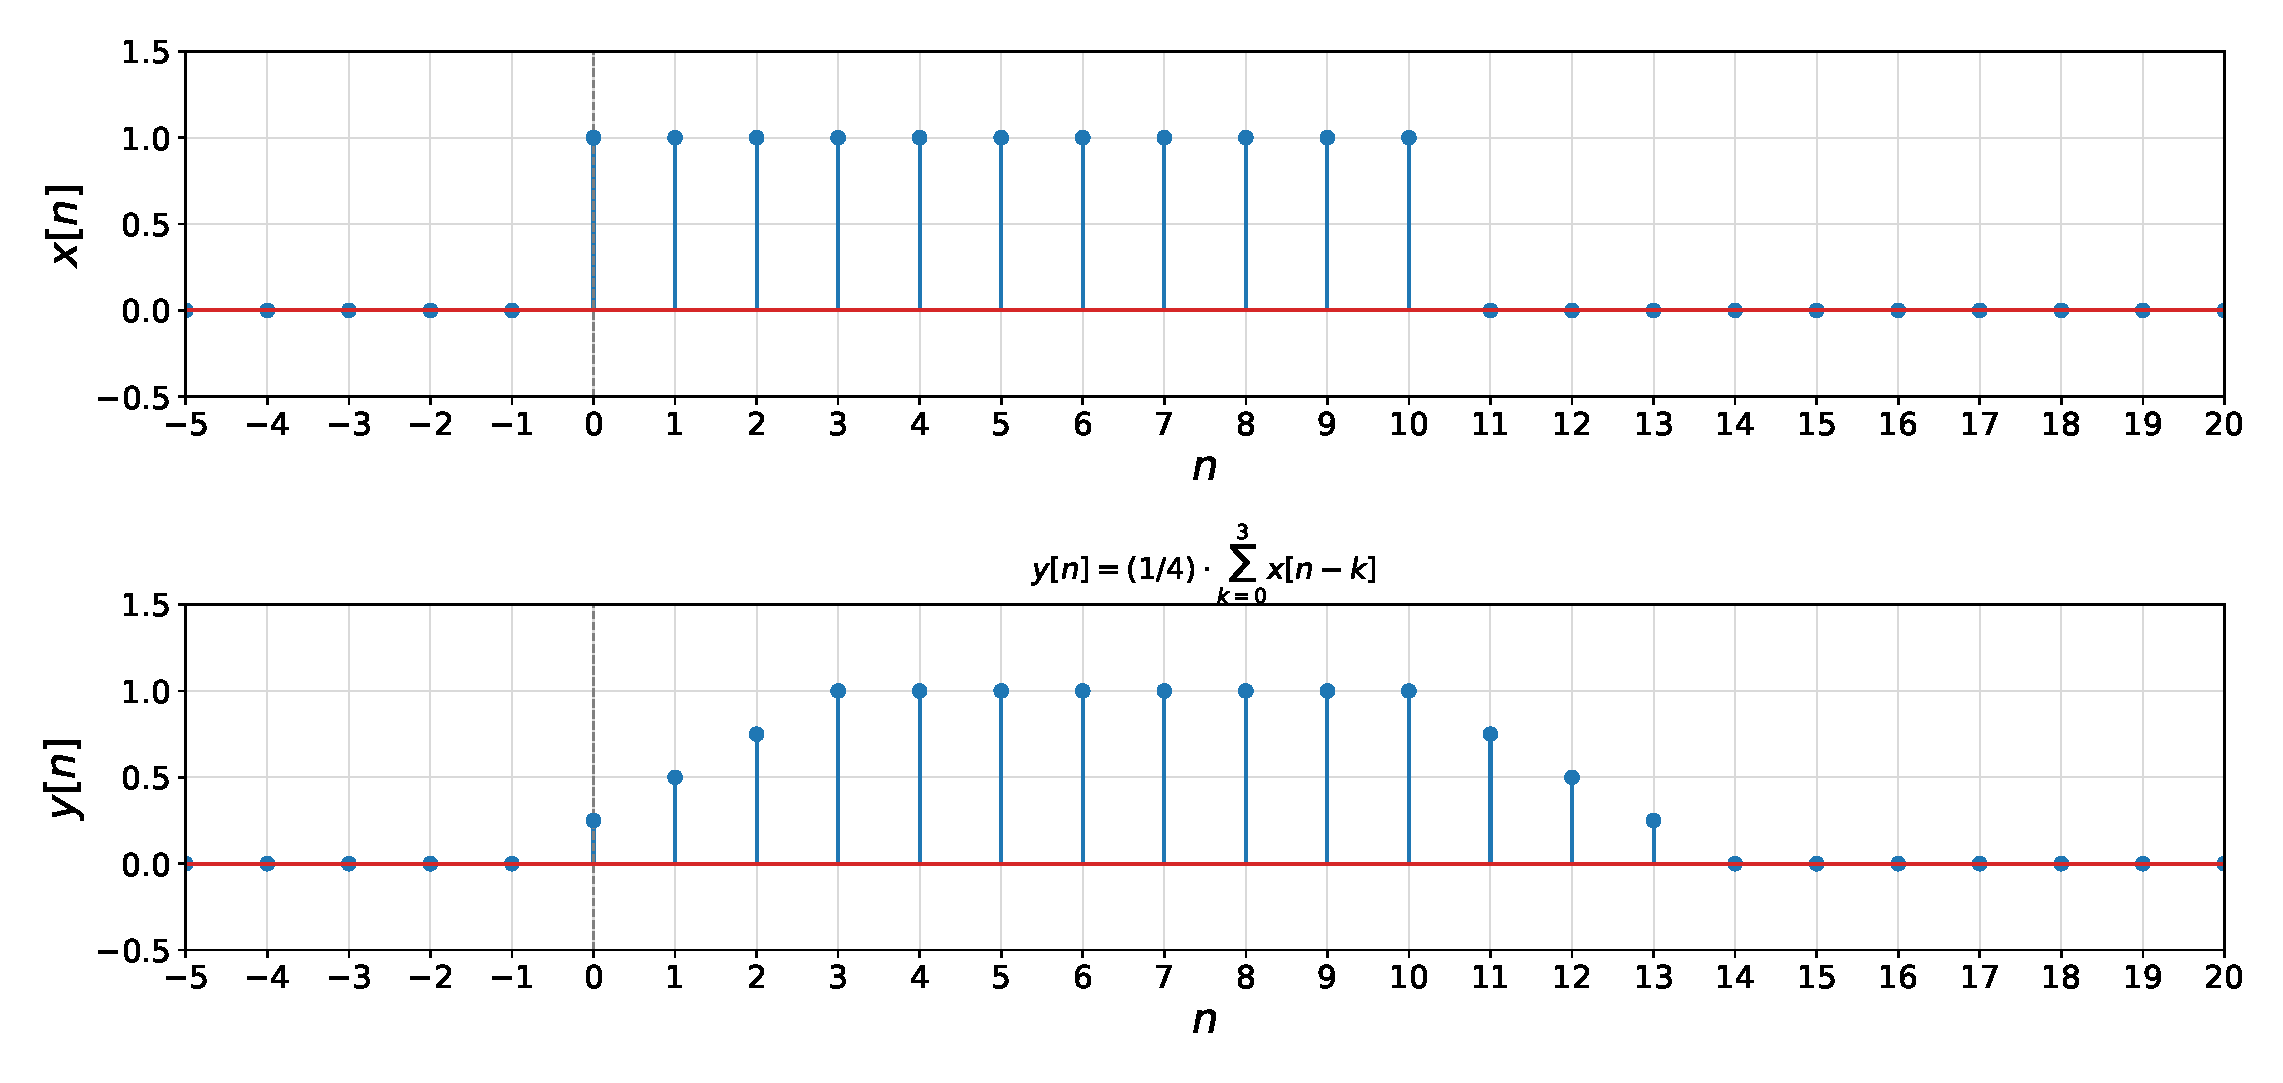
\includegraphics[width=\textwidth]{img/memory.eps}
% \end{figure}
% \end{frame}

% % CLASSIFICATION OF SYSTEMS
% \begin{frame}[t]{Classification of systems}

% \begin{itemize}
% \item \textbf{Causality}: \textit{a system whose output depends on the past and present only values of the input is a causal system}.
% \end{itemize}
% \end{frame}

% % CLASSIFICATION OF SYSTEMS
% \begin{frame}[t]{Classification of systems}
% \textbf{Causality}

% \begin{figure}
% 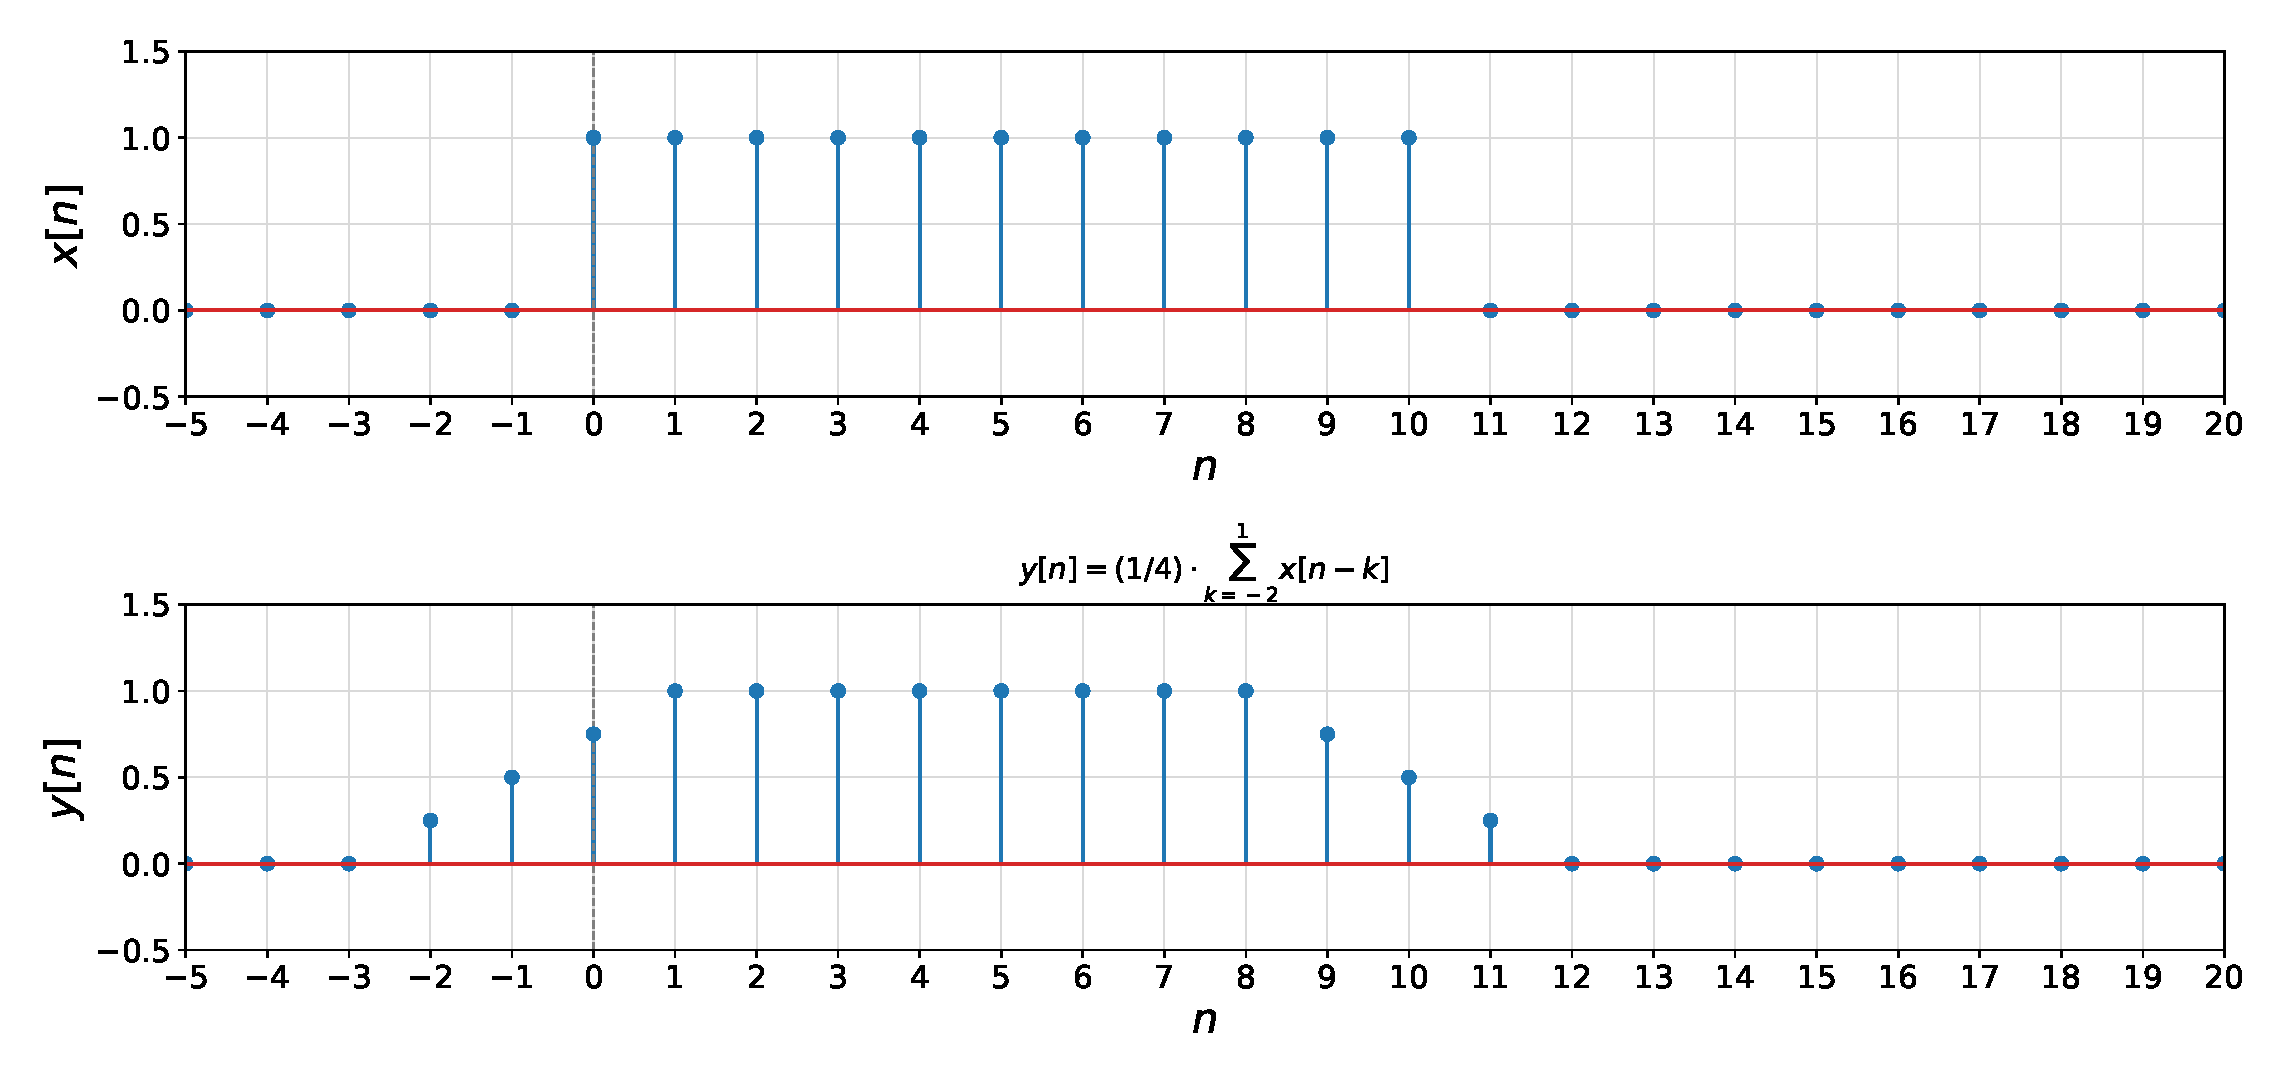
\includegraphics[width=\textwidth]{img/non-causal.eps}
% \end{figure}
% \end{frame}

% % CLASSIFICATION OF SYSTEMS
% \begin{frame}[t]{Classification of systems}

% \begin{itemize}
% \item \textbf{Time invariance}: \textit{system remains the same with time}.

% If a system is time-invariant, then
% \[ \mathcal{H}: x\ls n\rs \mapsto y\ls n\rs \iff f:x\ls n-k\rs \mapsto y\ls n-k\rs \]

% \end{itemize}
% \end{frame}


% % CLASSIFICATION OF SYSTEMS
% \begin{frame}[t]{Classification of systems}

% \begin{columns}[t]
%   \begin{column}{.45\linewidth}
%   \begin{figure}
%   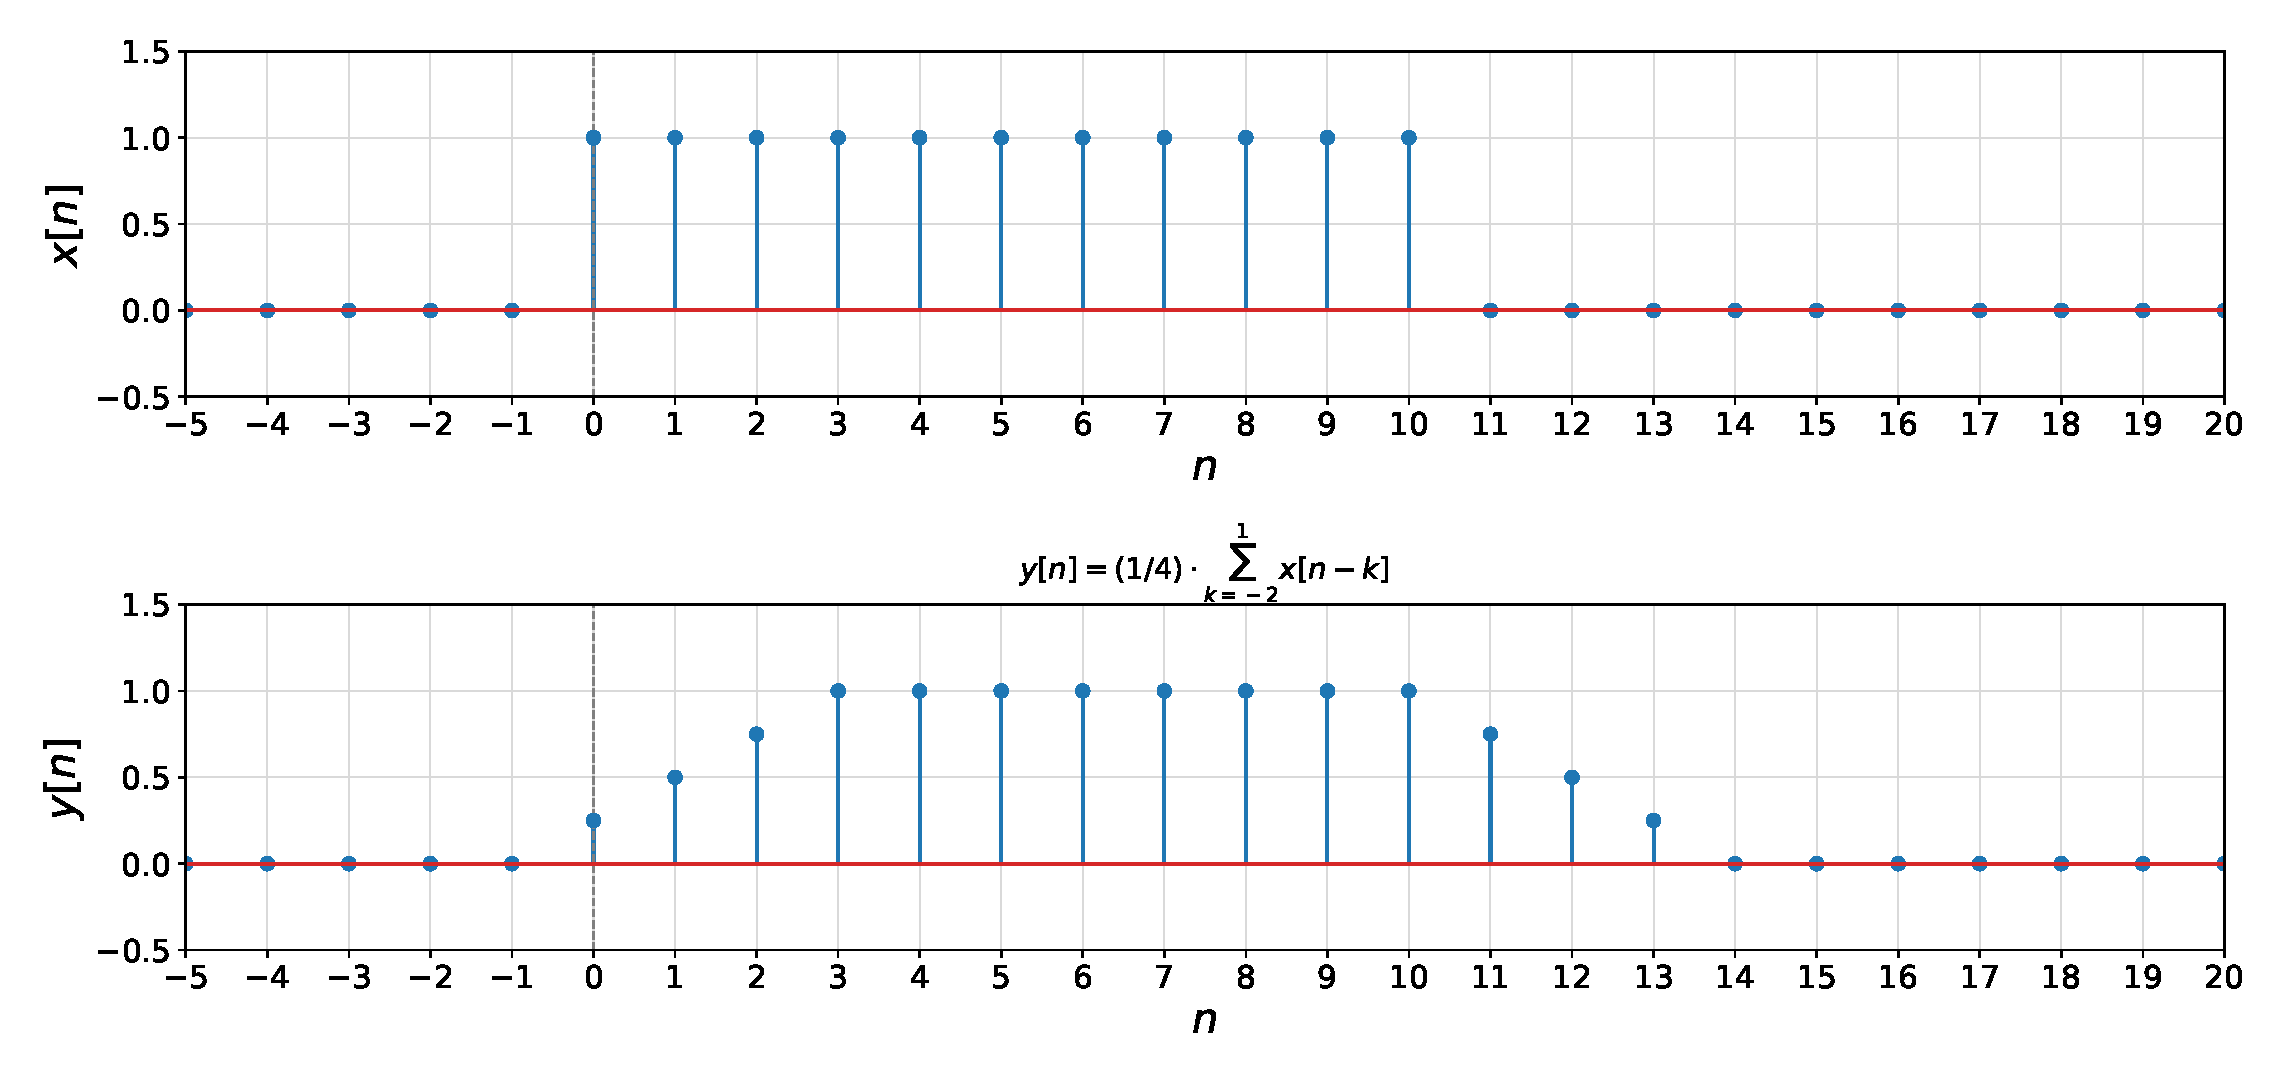
\includegraphics[width=\textwidth]{img/timeinvar1.eps}
%   \end{figure}
%   \end{column}

%   \begin{column}{.45\linewidth}
%   \begin{figure}
%   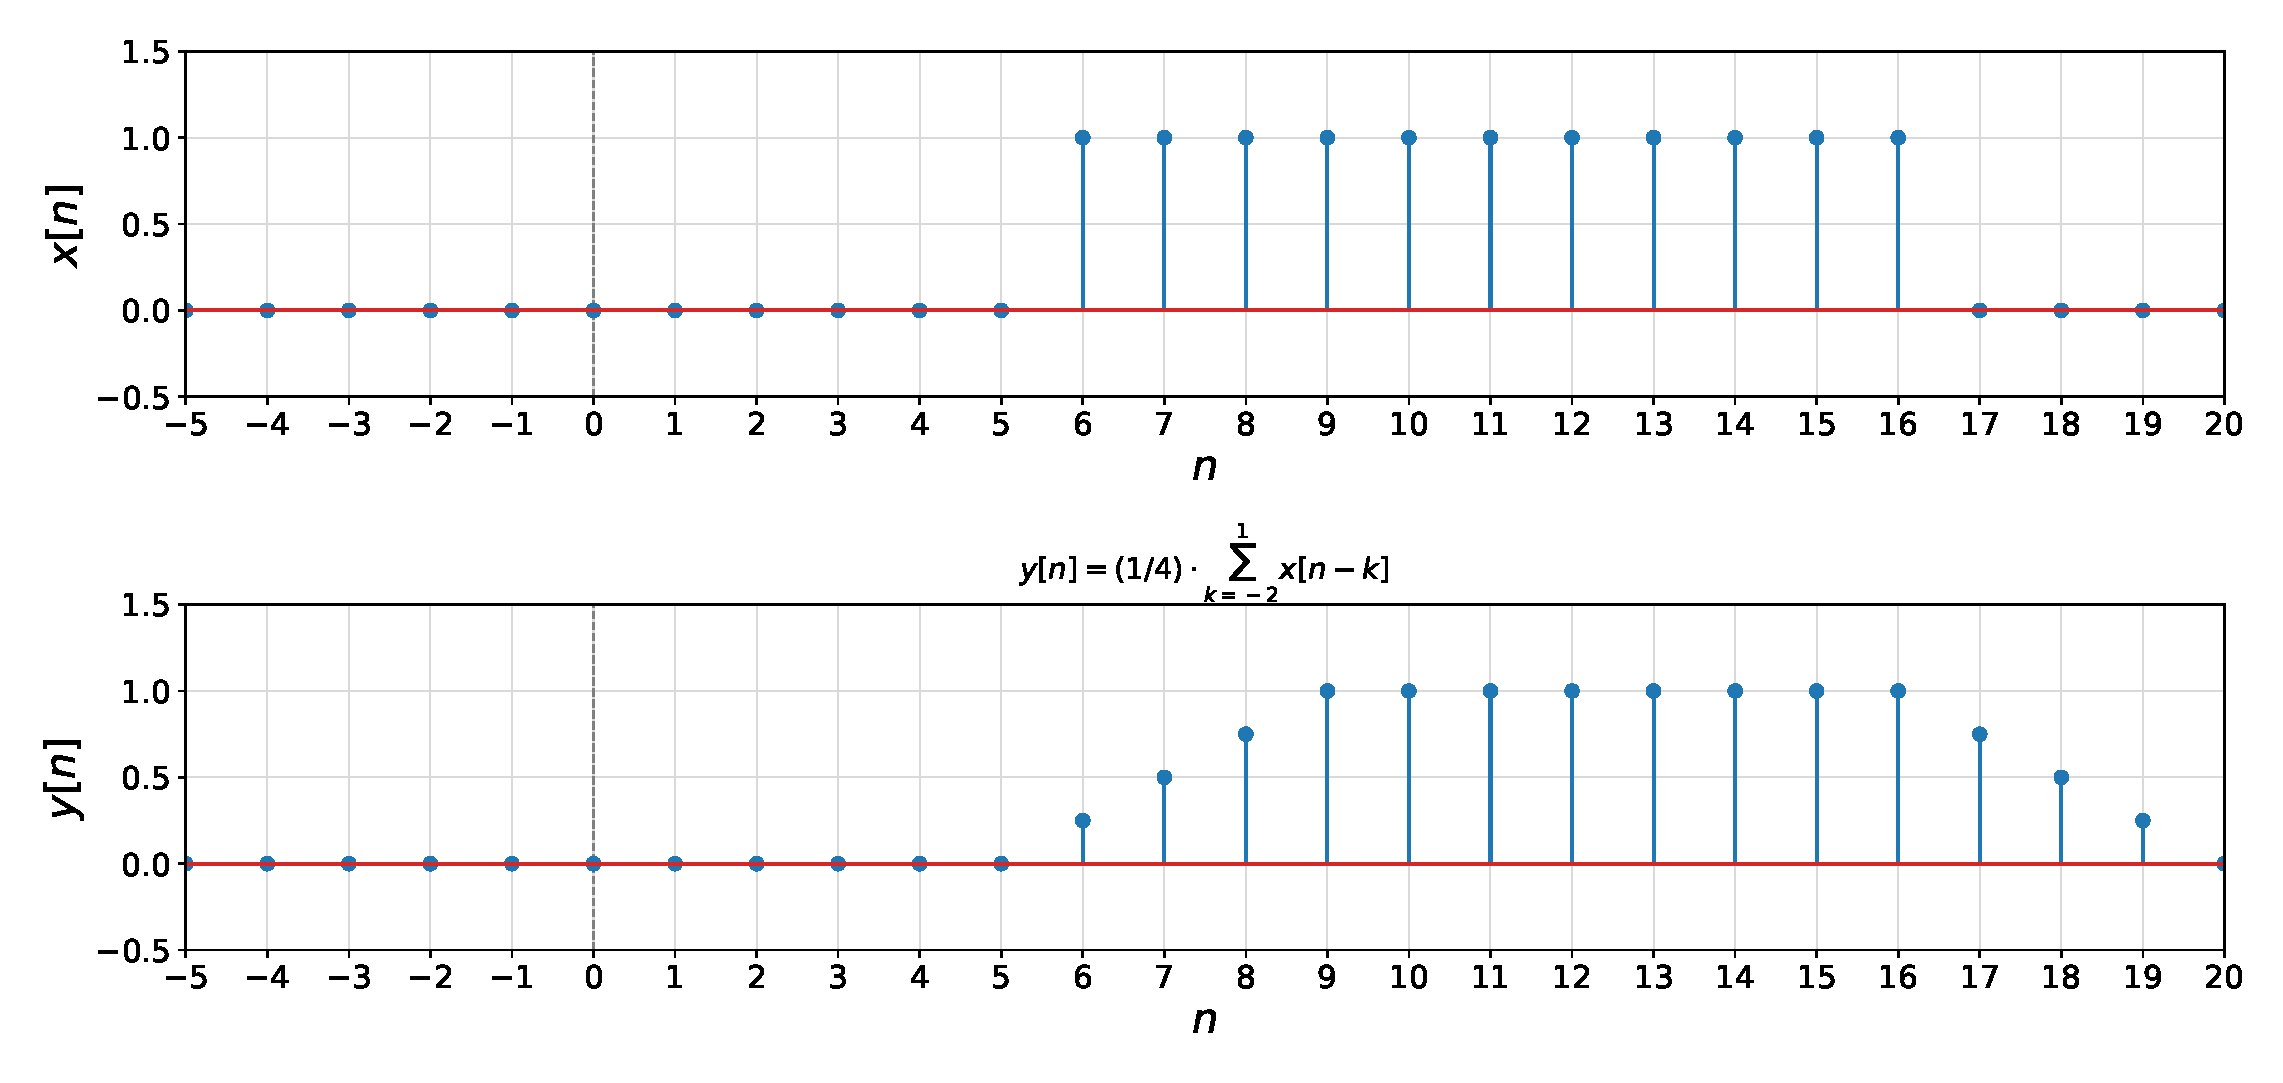
\includegraphics[width=\textwidth]{img/timeinvar2.eps}
%   \end{figure}
%   \end{column}
% \end{columns}
% \end{frame}


% % CLASSIFICATION OF SYSTEMS
% \begin{frame}[t]{Classification of systems}

% \begin{columns}[t]
%   \begin{column}{.45\linewidth}
%   \begin{figure}
%   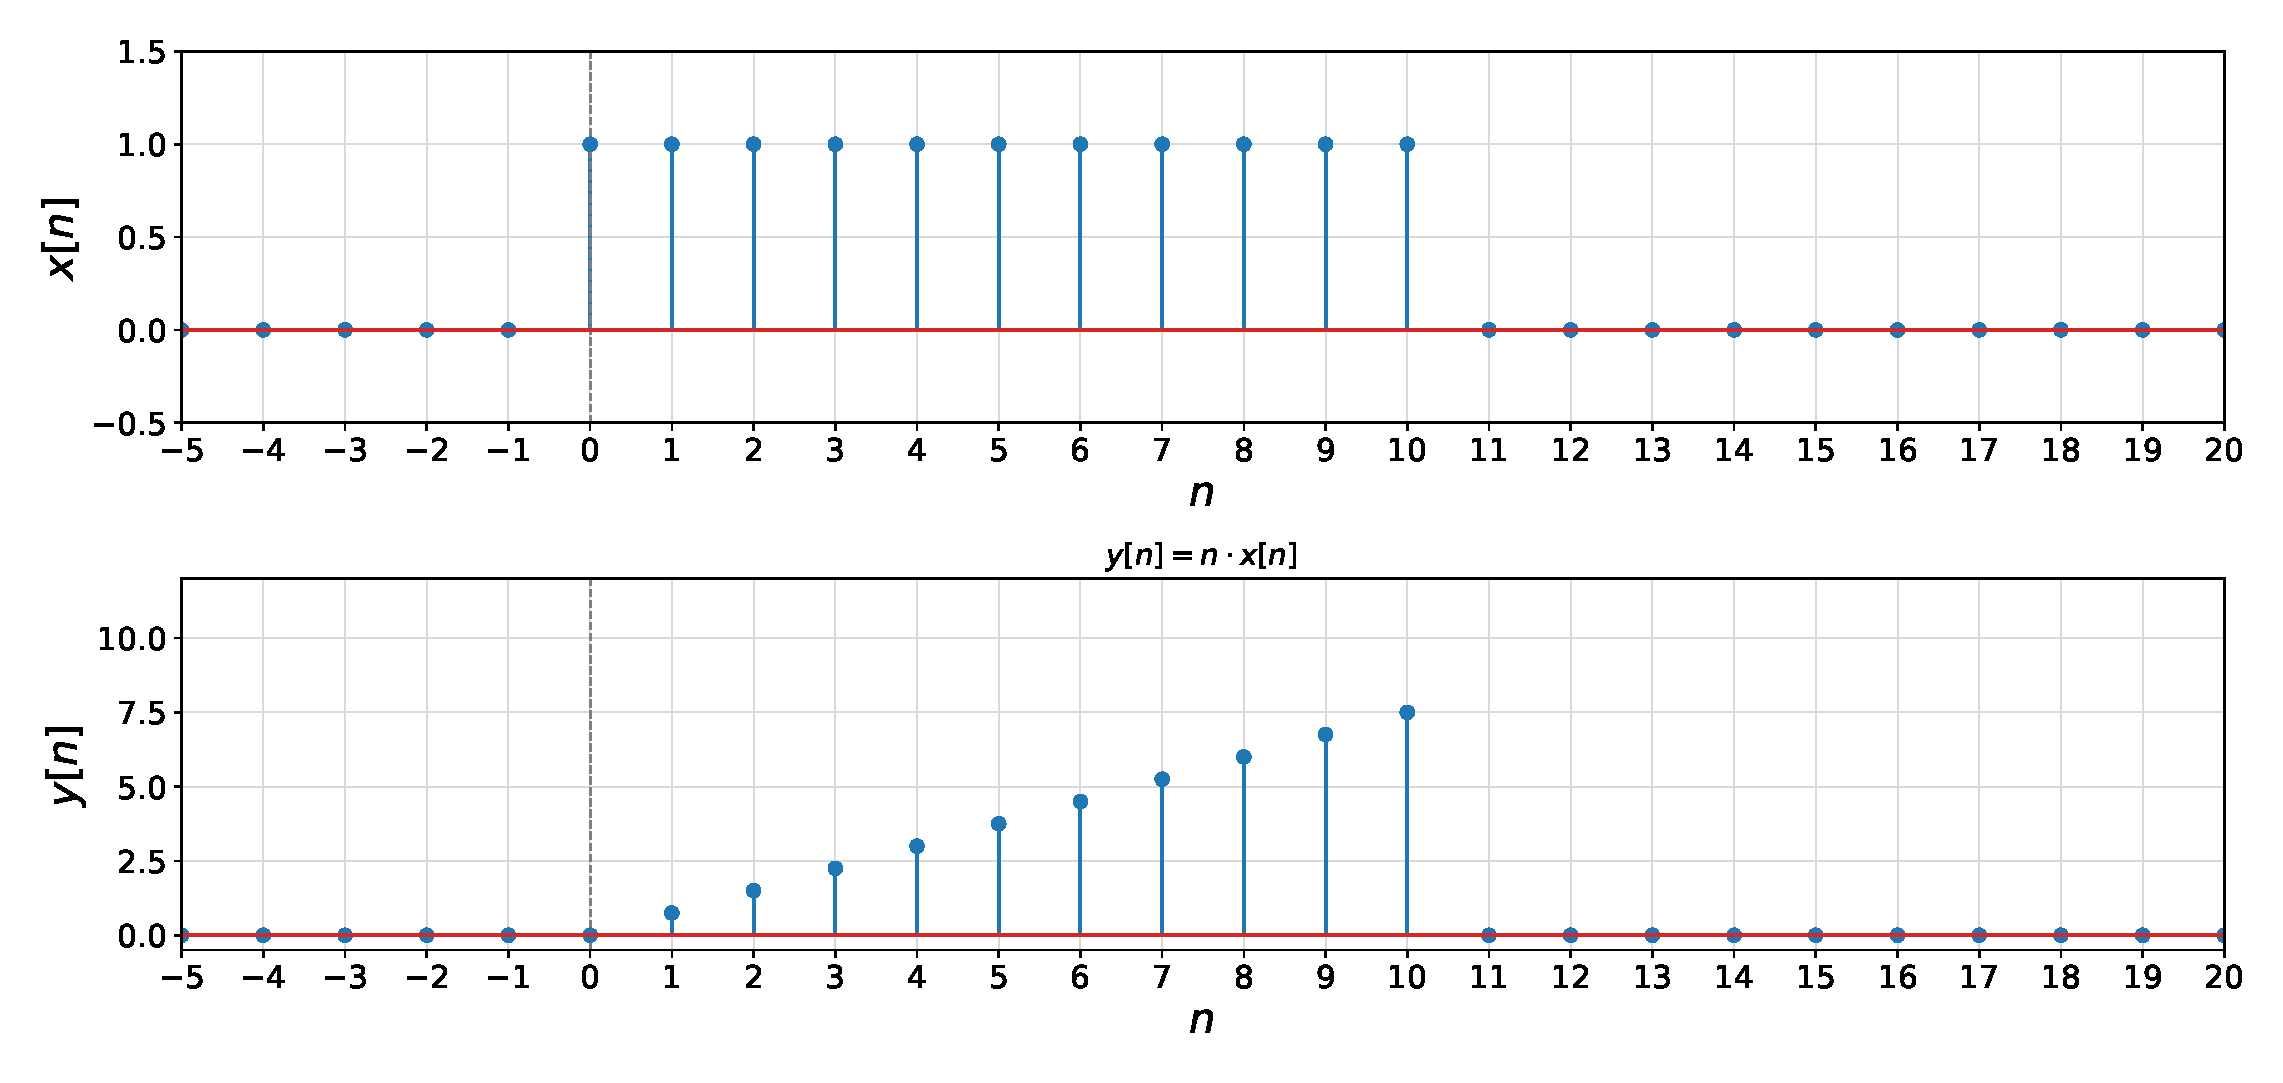
\includegraphics[width=\textwidth]{img/timevar1.eps}
%   \end{figure}
%   \end{column}

%   \begin{column}{.45\linewidth}
%   \begin{figure}
%   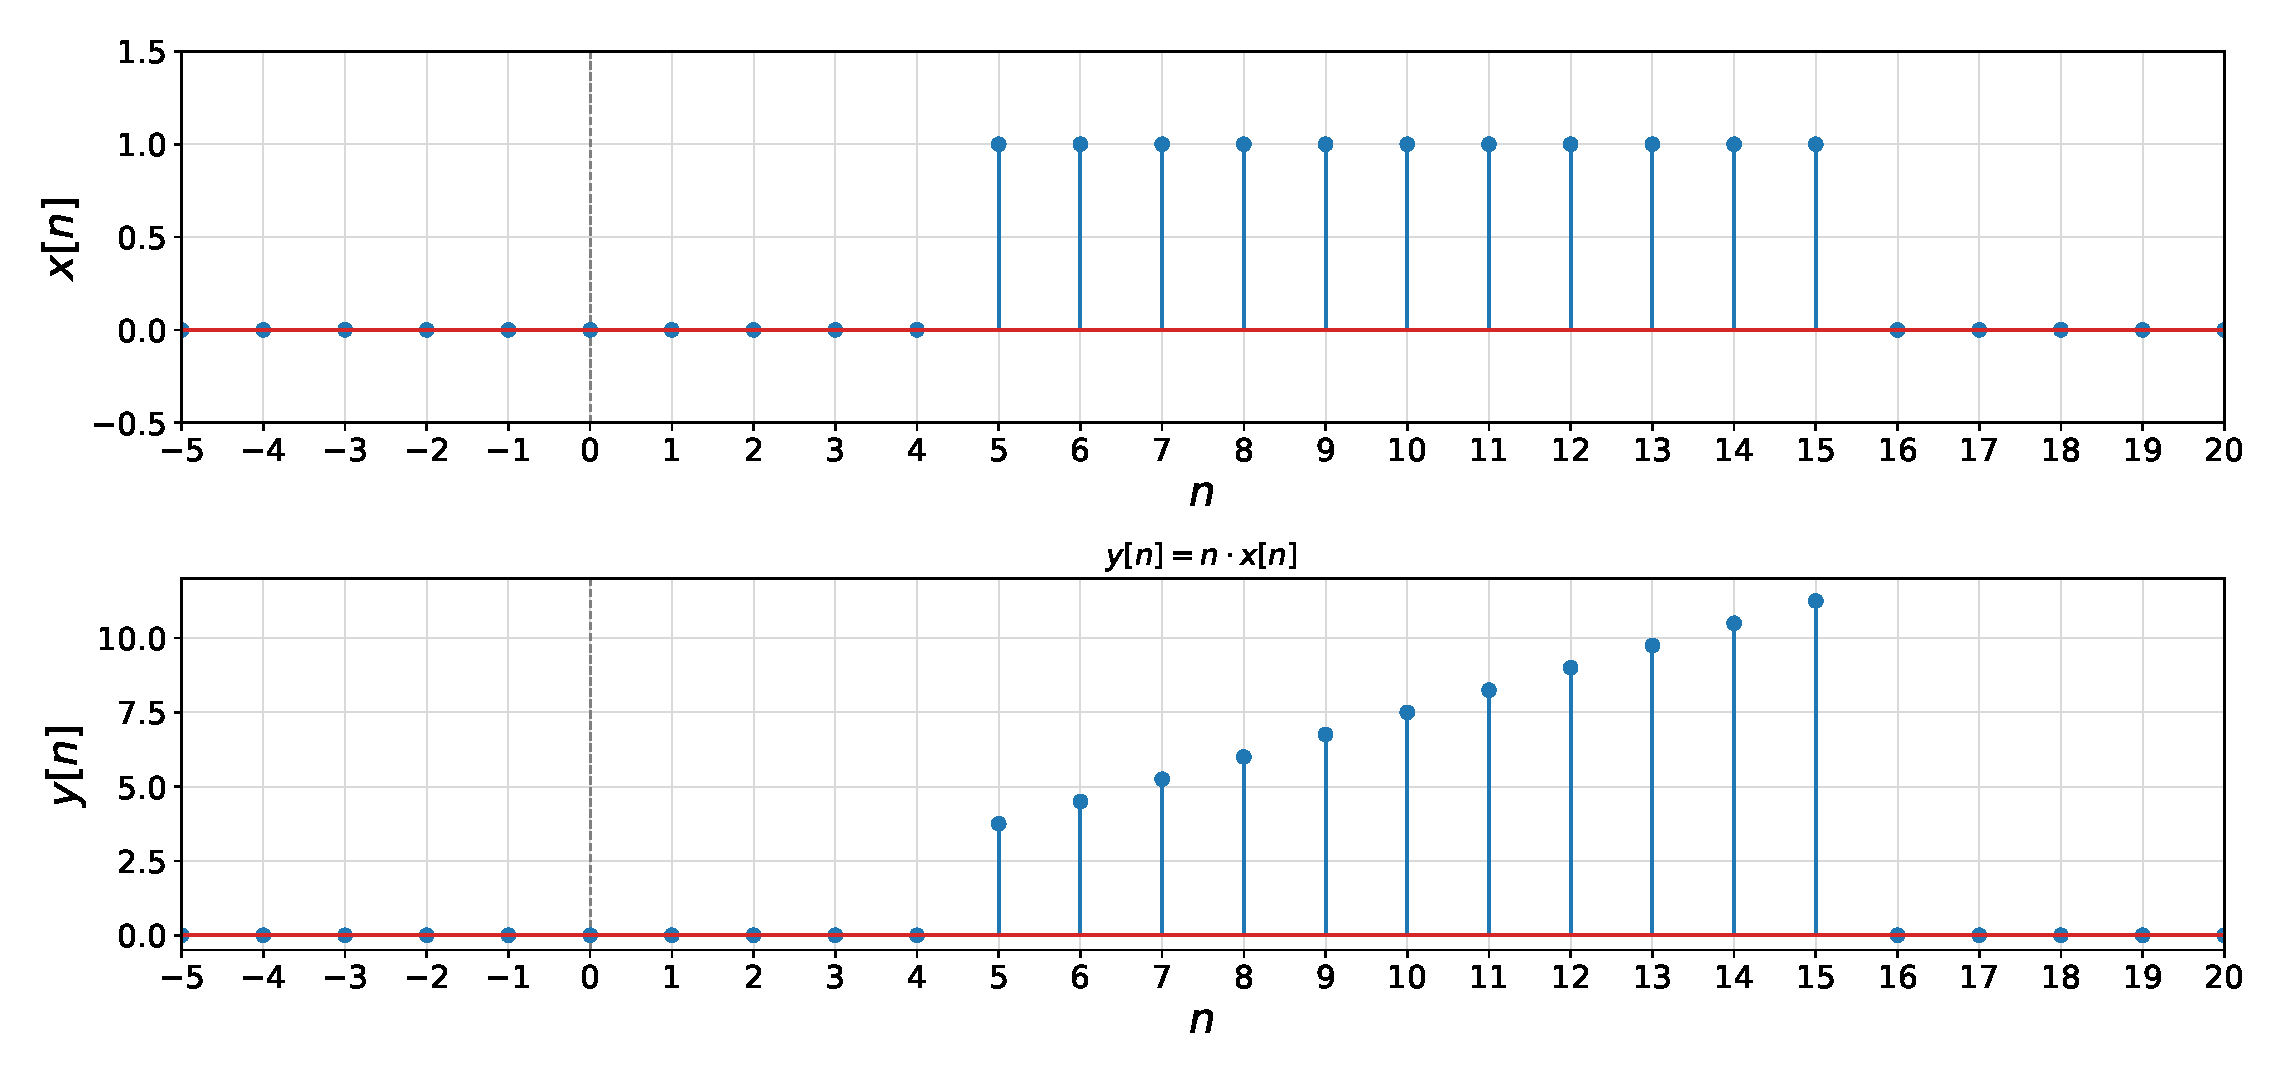
\includegraphics[width=\textwidth]{img/timevar2.eps}
%   \end{figure}
%   \end{column}
% \end{columns}
% \end{frame}


% % CLASSIFICATION OF SYSTEMS
% \begin{frame}[t]{Classification of systems}

% \begin{itemize}
% \item \textbf{Stability}: \textit{bounded input produces bounded output}.

% \[ \left|x\ls n \rs\right| < M_x < \infty \mapsto \left|y\ls n \rs\right| < M_y < \infty \]
% \end{itemize}
% \end{frame}

\end{document}